\chapter{Results}

%	<Paragraph> Overview of results
This chapter presents results of the $k$-{\sc Sat} execution test from the previous chapter.  We consider the results of the test and analyze the algorithm metrics.  

	\section{Algorithm metric comparison}
	
%		<Paragraph> Summary of measured metrics
This section describes the results from the simulation.  We analyze the molecular operations count for append, extract, mix, purify, splice, and split.  Presentation of actual computation time and required memory for the solution representation allow for comparison of algorithms.

%\subsection{Split}
%%%%%%%%%%%%%%%%%%%%%%%%%%%%%%%%%
\begin{figure}[htdp]

\begin{center}

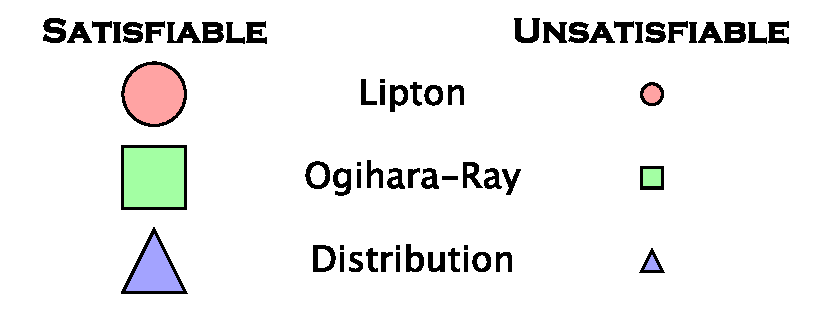
\includegraphics[width=0.8\textwidth]{./figures/key.pdf}

\caption{Key for output metrics.  Large shapes represent satisfiable instances and small shapes represent unsatisfiable instances.  Datapoints for Lipton's algorithm are represented with red circles, Ogihara and Ray's algorithm with green squares, and the Distribution algorithm with blue triangles. }
\label{metricKey}
\end{center}
\end{figure}
%%%%%%%%%%%%%%%%%%%%%%%%%%%%%%%%%
\FloatBarrier

%\subsection{Append}
%%%%%%%%%%%%%%%%%%%%%%%%%%%%%%%%%
\begin{figure}[htdp]

\reversemarginpar{
\textbf{Append} concatenates two oligonucleotides. \\

The Distribution algorithm is exponential in the number of appends.  The operation count for append depends on the parsing order of the CNF instance.\\

Lipton's and Ogihara-Ray's algorithms use a fixed number of appends.  This depends on the number of variables and clauses present in the CNF instance.
}

\begin{center}

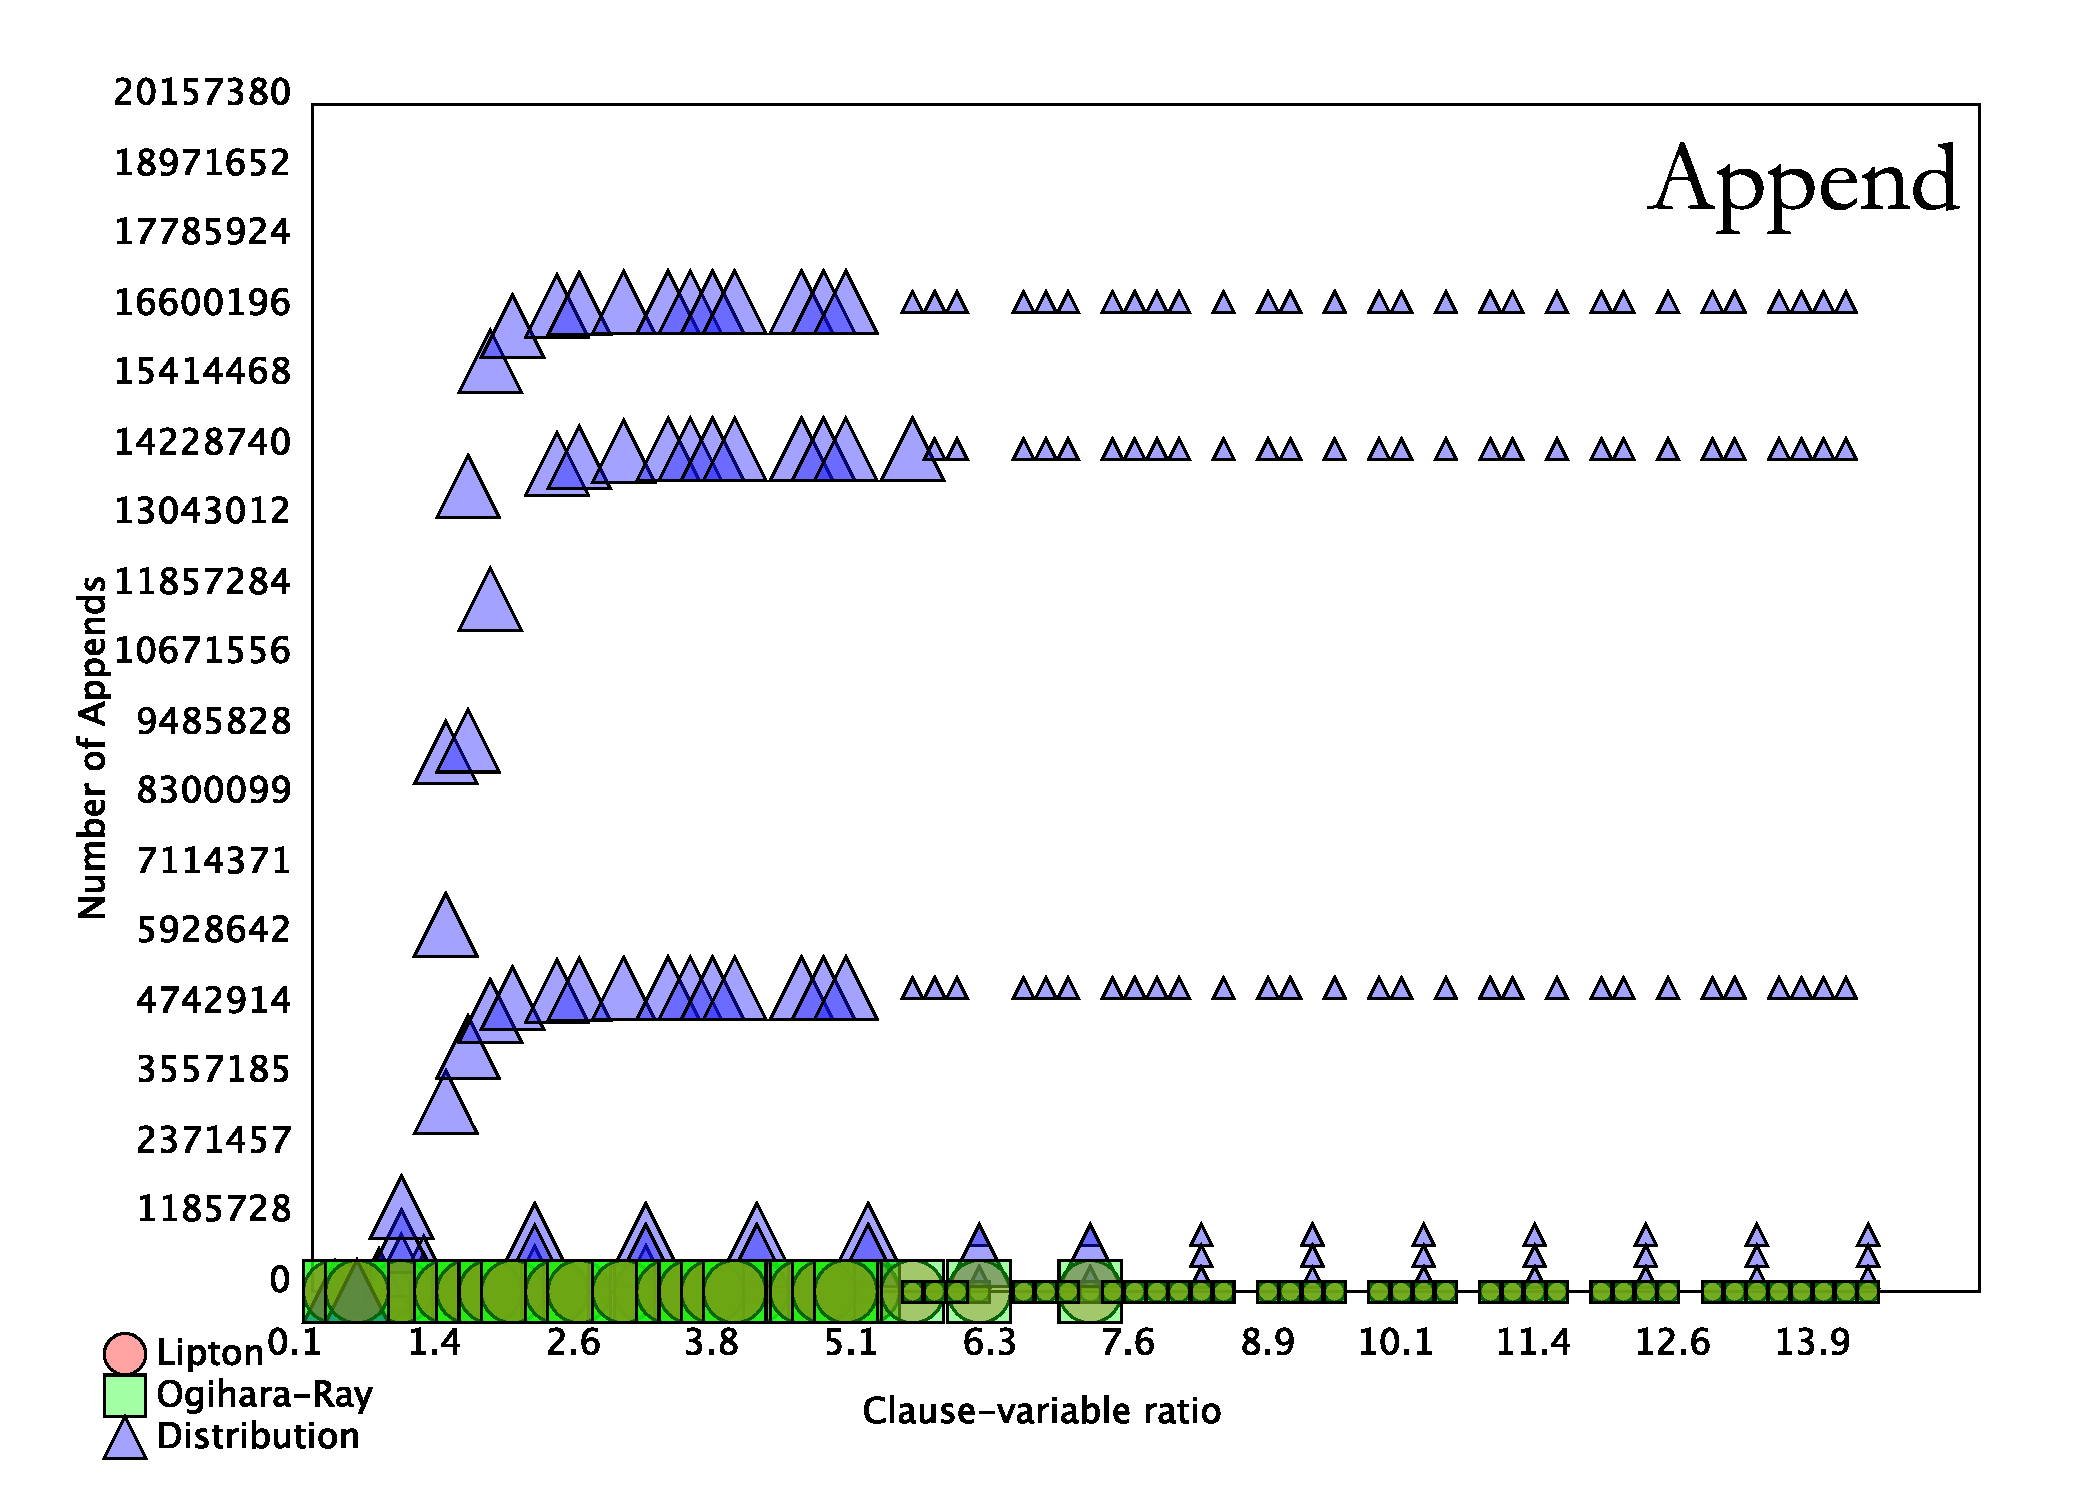
\includegraphics[width=1.1\textwidth]{./figures/metricOutput/Append.pdf}

\caption{Clause to variable ratio $\alpha$ vs. Number of appends }
\label{appendFig}
\end{center}
\end{figure}
%%%%%%%%%%%%%%%%%%%%%%%%%%%%%%%%%

\FloatBarrier
			
%\subsection{Extract}
%%%%%%%%%%%%%%%%%%%%%%%%%%%%%%%%%
\begin{figure}[htdp]

\reversemarginpar{

\textbf{Extract} filters oligonucleotides from a tube.\\

Ogihara-Ray's algorithm requires the greatest number of extracts.  Lipton's algorithm is linear on $\alpha$ and varies a constant from Ogihara-Ray's algorithm.\\

The Distribution algorithm does not require extract.

}

\begin{center}

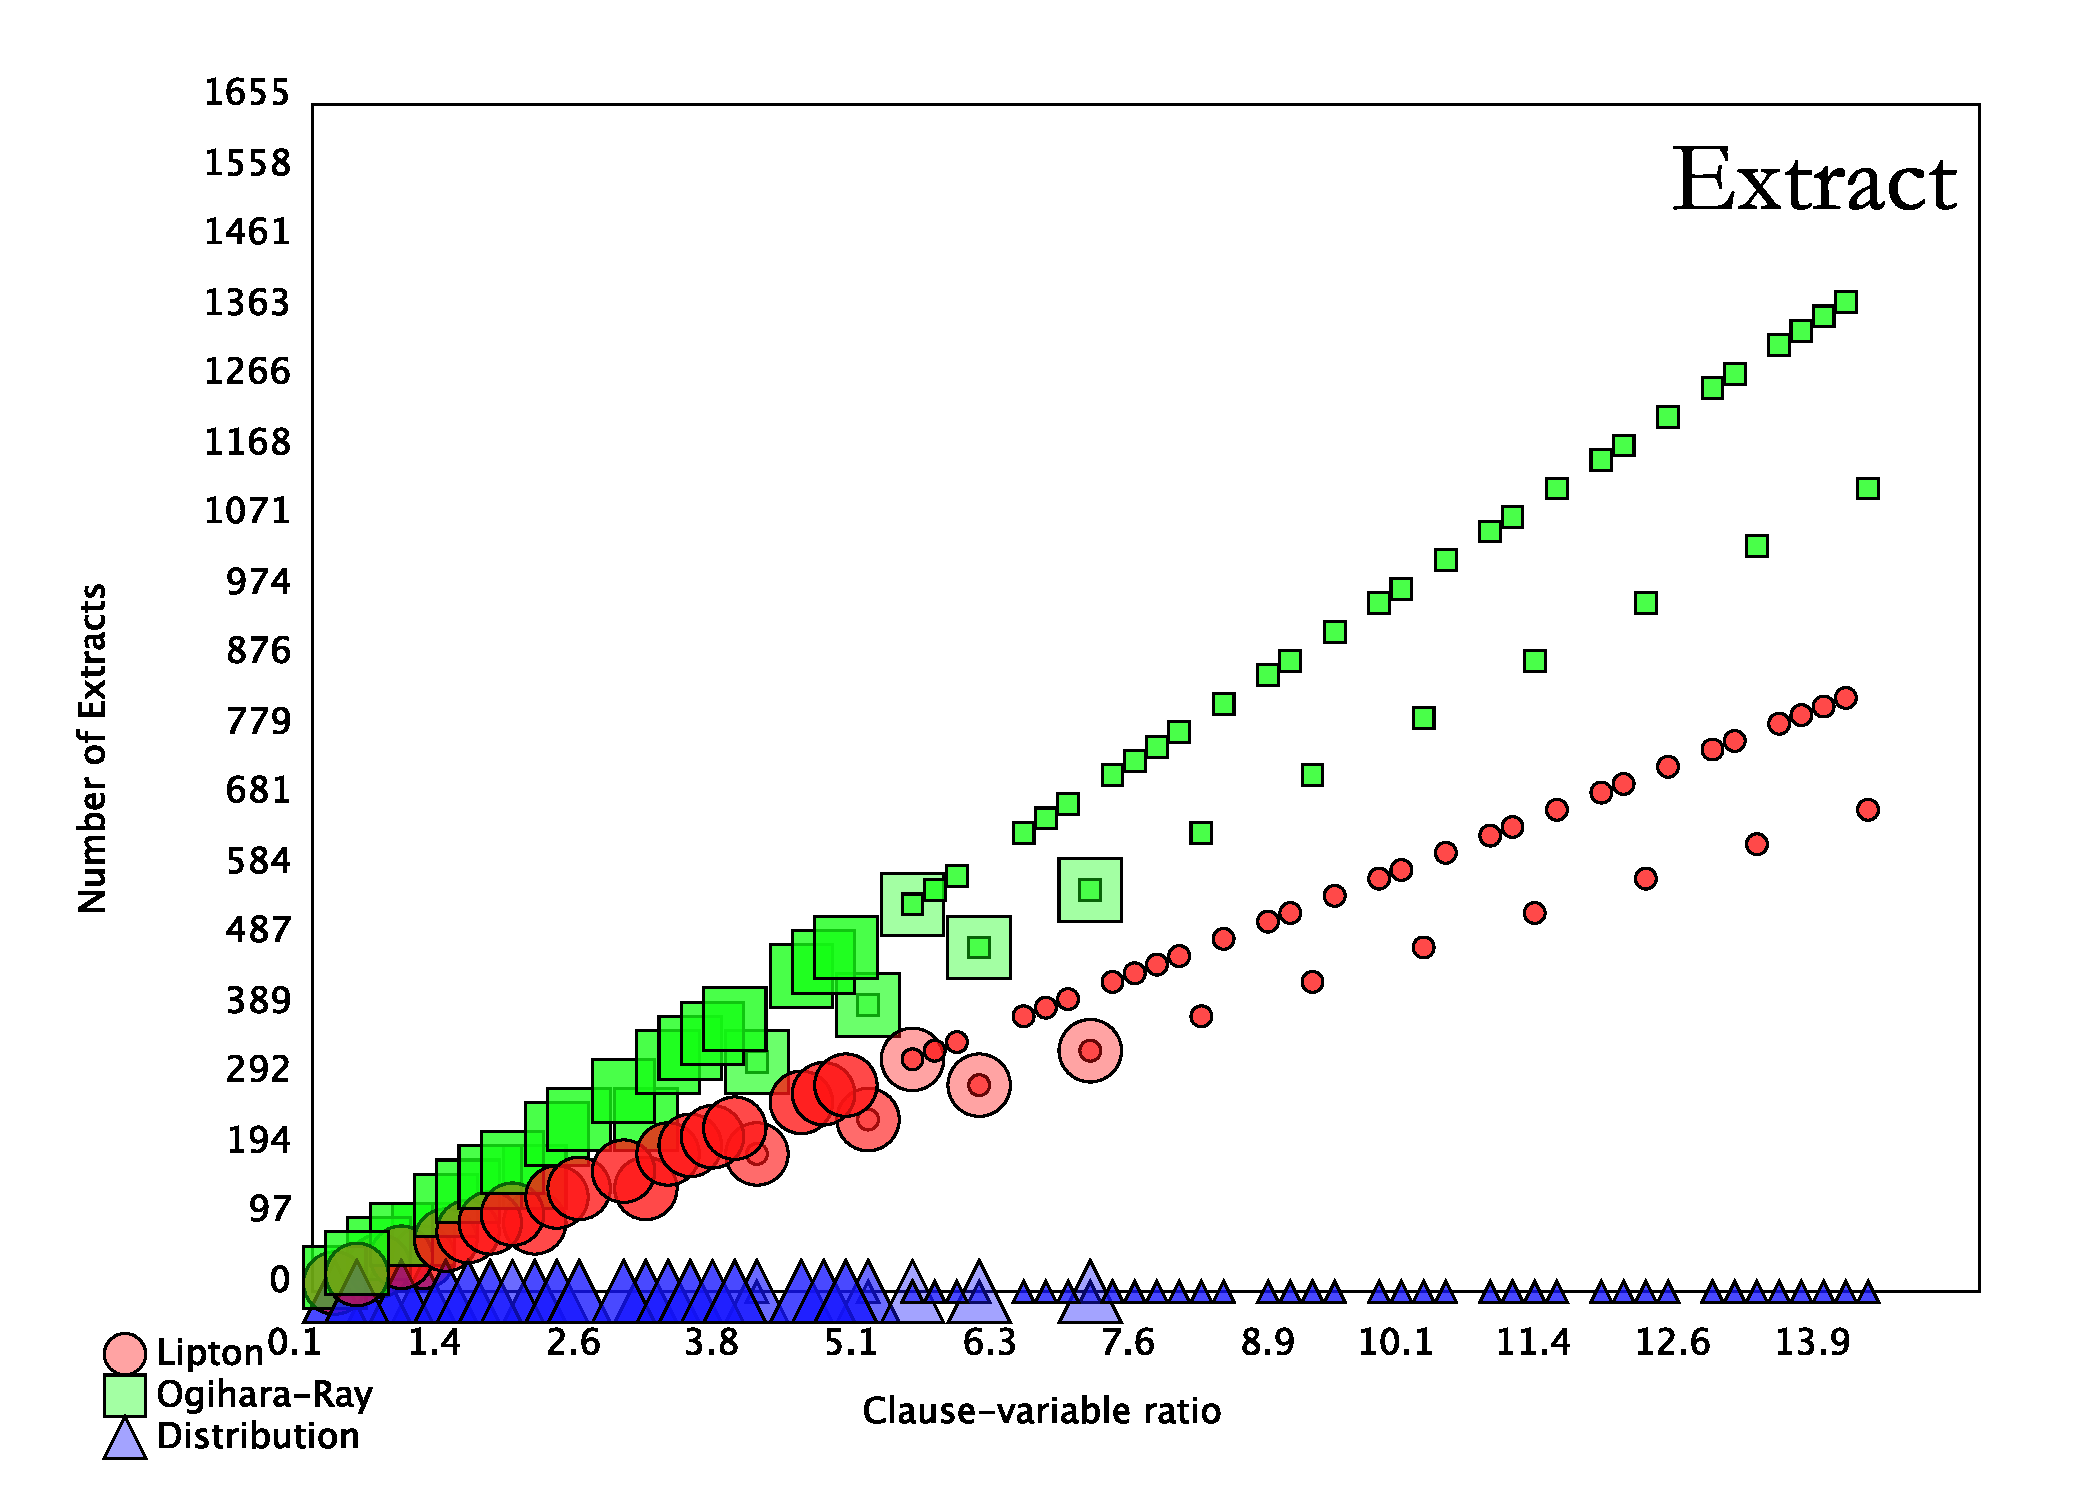
\includegraphics[width=1.1\textwidth]{./figures/metricOutput/Extract.pdf}

\caption{Clause to variable ratio $\alpha$ vs. Number of extracts }
\label{extractFig}
\end{center}
\end{figure}
%%%%%%%%%%%%%%%%%%%%%%%%%%%%%%%%%
\FloatBarrier			
			
%\subsection{Mix}
%%%%%%%%%%%%%%%%%%%%%%%%%%%%%%%%%
\begin{figure}[htdp]

\reversemarginpar{
\textbf{Mix} combines the contents of two tubes.\\

Lipton's algorithm requires a linear number of mixes on $\alpha$.  The Distribution algorithm also requires a linear number of mixes, varying by a constant factor from Lipton's algorithm.\\

Ogihara-Ray's algorithm requires a constant number of mixes on $\alpha$.
}

\begin{center}

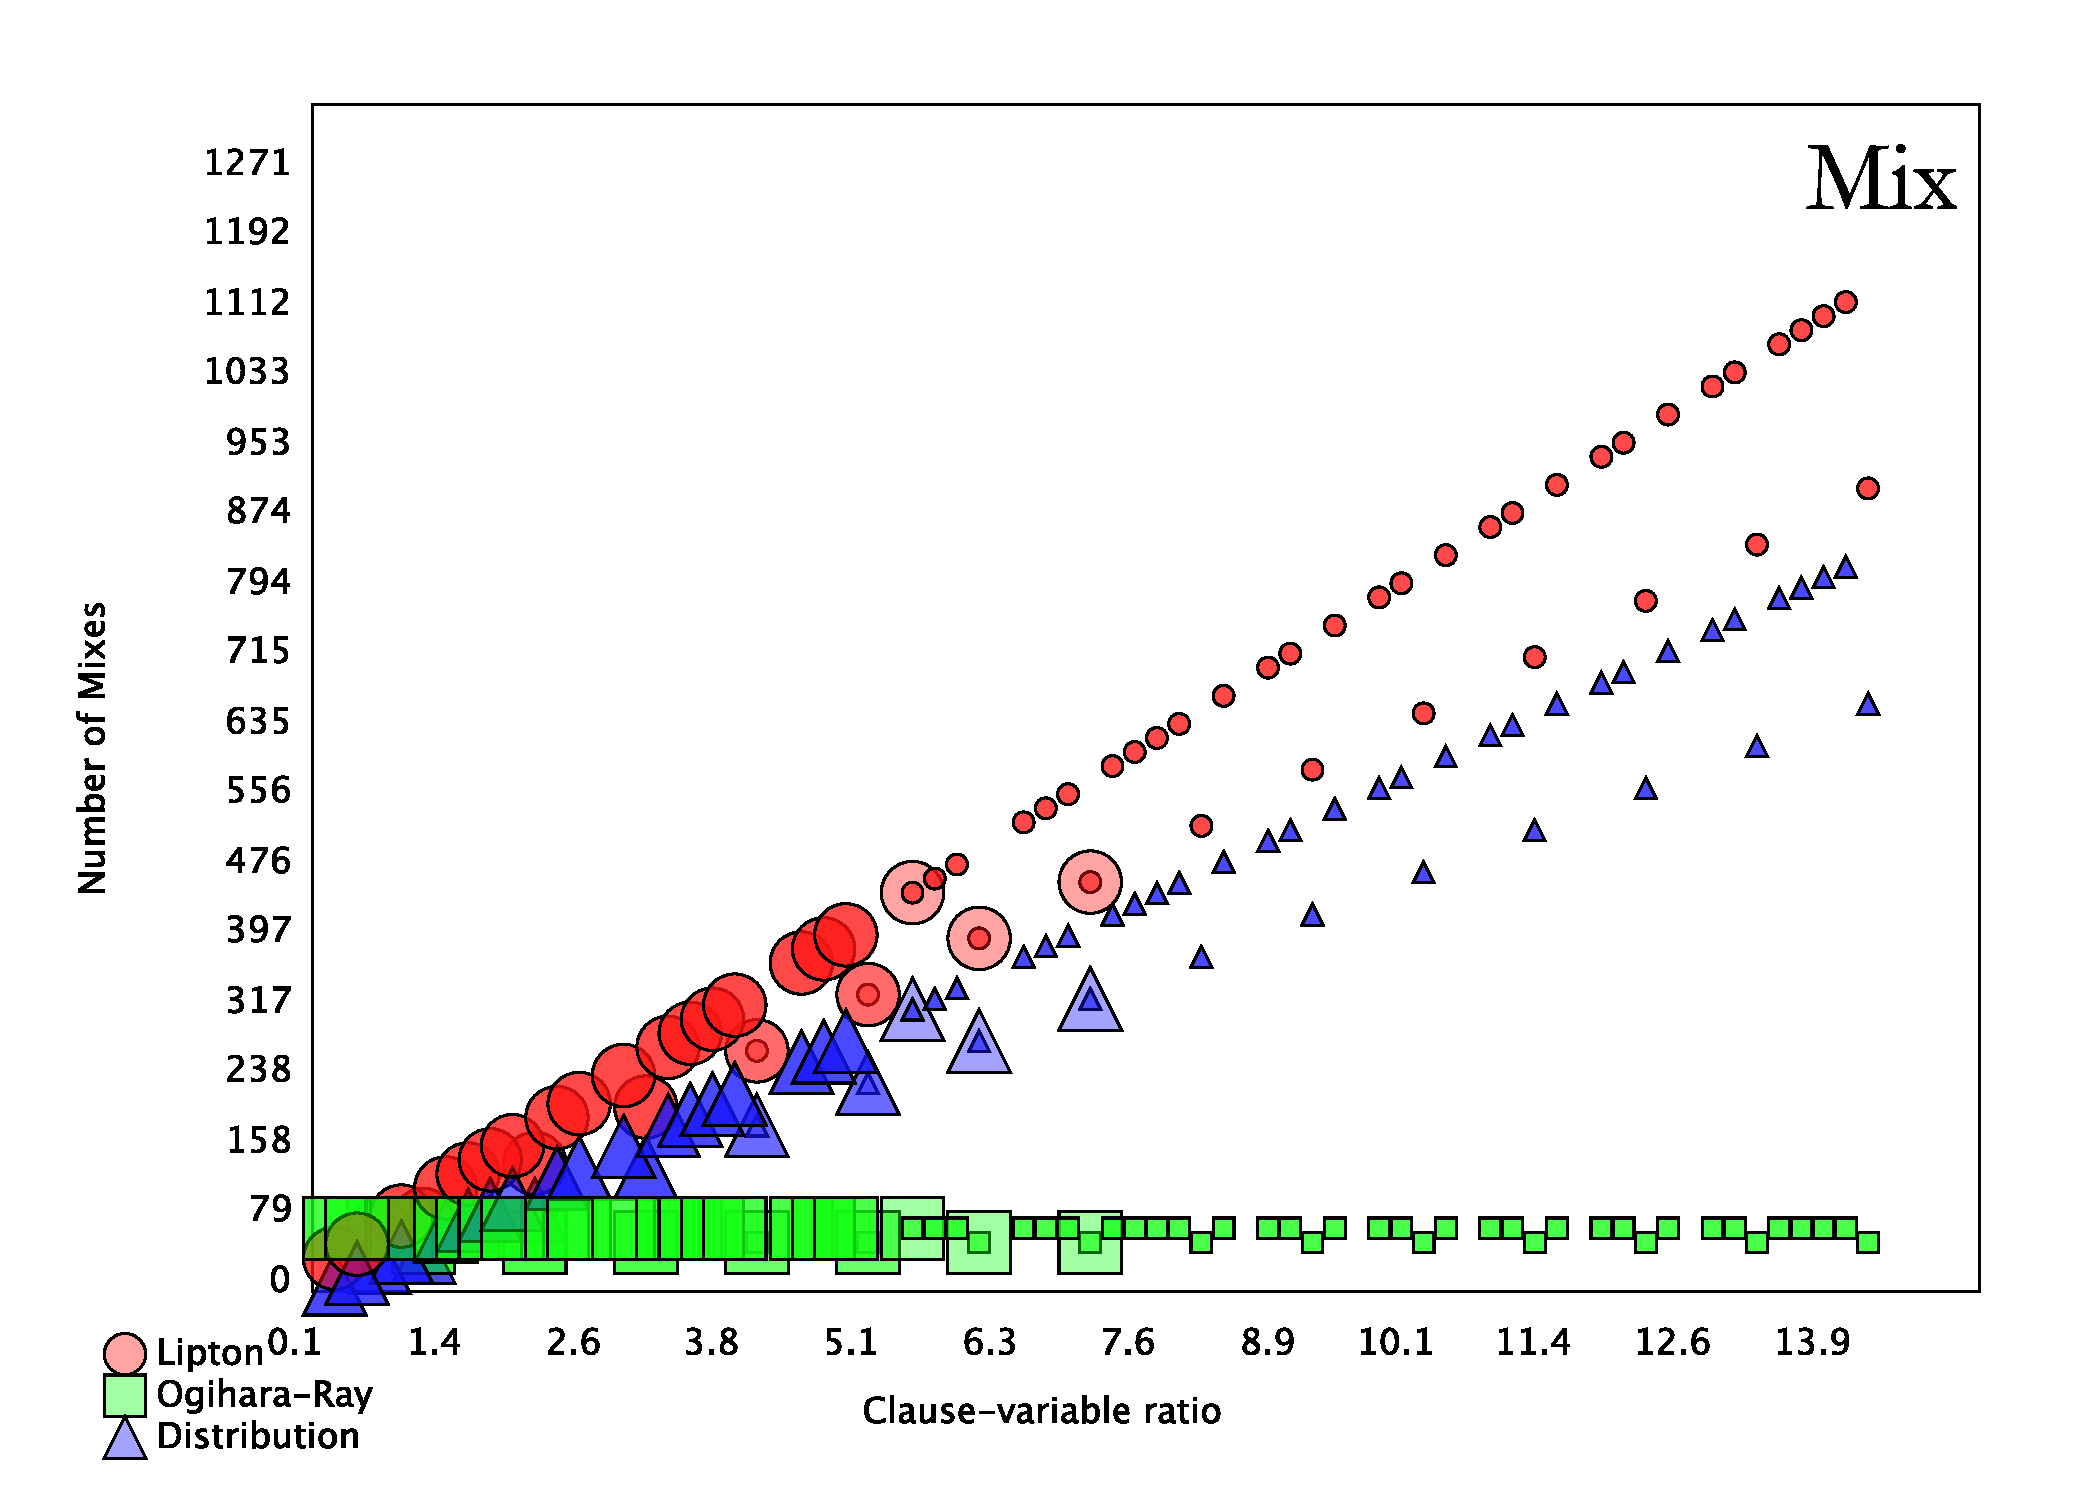
\includegraphics[width=1.1\textwidth]{./figures/metricOutput/Mix.pdf}

\caption{Clause to variable ratio $\alpha$ vs. Number of mixes }
\label{mixFig}
\end{center}
\end{figure}
%%%%%%%%%%%%%%%%%%%%%%%%%%%%%%%%%
\FloatBarrier

%\subsection{Purify}
%%%%%%%%%%%%%%%%%%%%%%%%%%%%%%%%%
\begin{figure}[htdp]

\reversemarginpar{
\textbf{Purify} ensures a uniform distribution of each independent oligonucleotide in a tube.\\

All three algorithms operate using a linear number of purifications on $\alpha$.  Ogihara-Ray's algorithm requires the greatest number of purifications.  The purifications vary by a constant when compared to Lipton's and the Distribution algorithms.

 }

\begin{center}

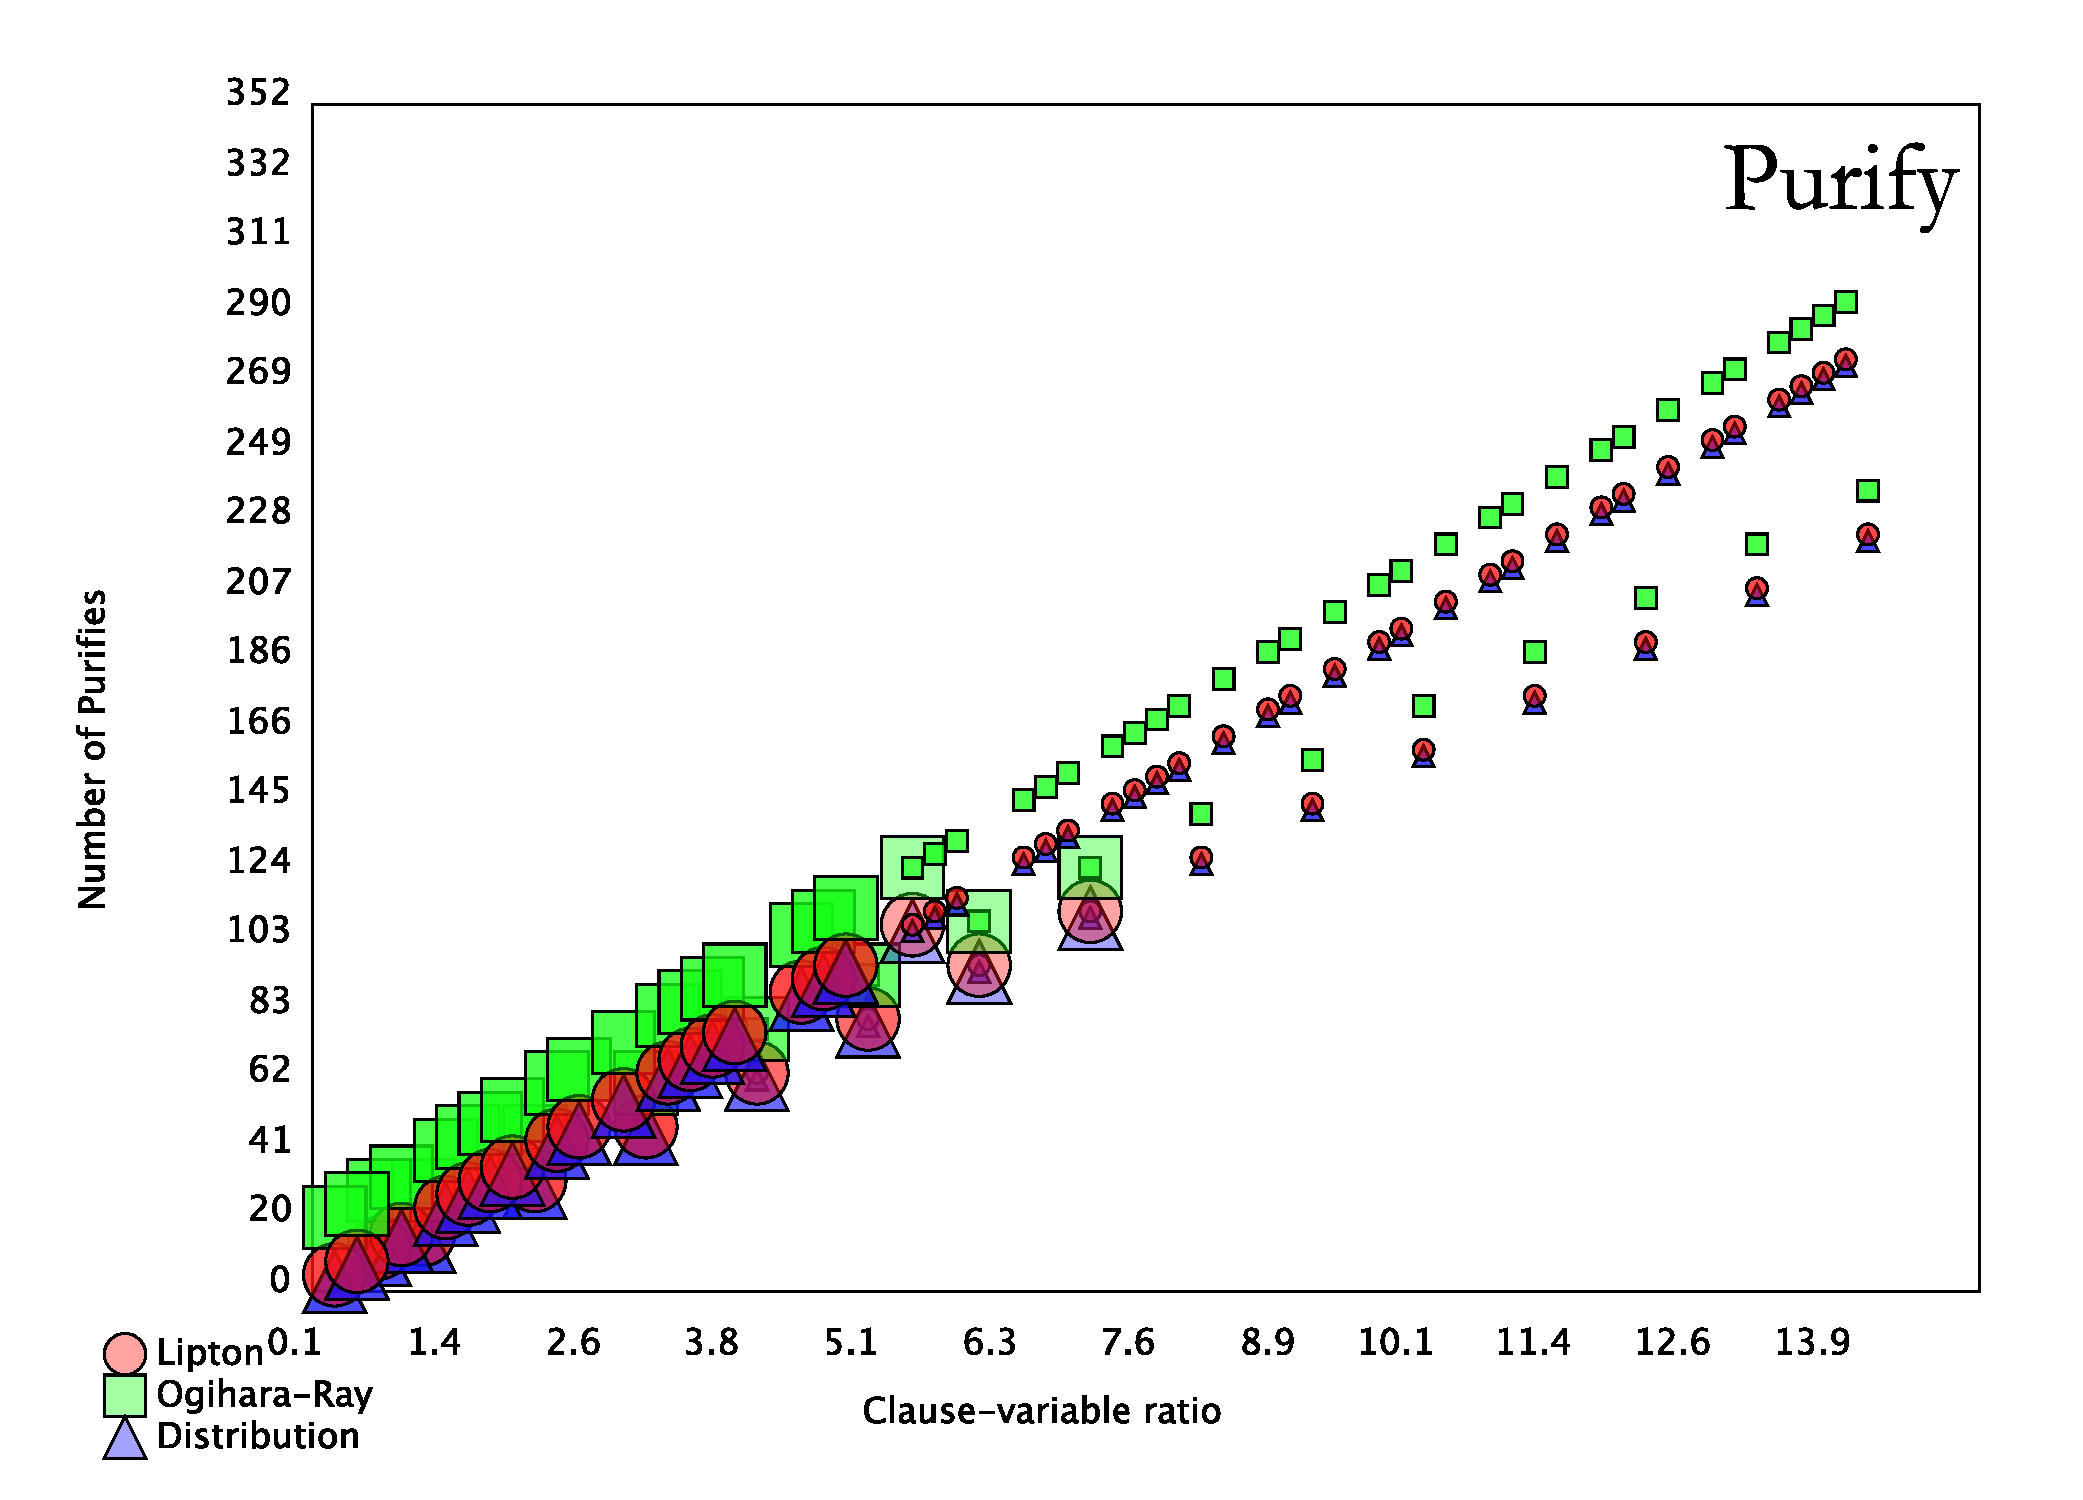
\includegraphics[width=1.1\textwidth]{./figures/metricOutput/Purify.pdf}

\caption{Clause to variable ratio $\alpha$ vs. Number of purifies }
\label{purifyFig}
\end{center}
\end{figure}
%%%%%%%%%%%%%%%%%%%%%%%%%%%%%%%%%
\FloatBarrier

%\subsection{Splice}
%%%%%%%%%%%%%%%%%%%%%%%%%%%%%%%%%
\begin{figure}[htdp]

\reversemarginpar{
\textbf{Splice} cuts an oligonucleotide at a targeted location.\\

The Distribution algorithm is exponential in the number of splices.  The number of splices depends on the parsing order of the CNF instance.  Each split requires reassembly, accomplished using two appends.  Figure \ref{appendFig} shows the number of appends.\\

Lipton's and Ogihara-Ray's algorithms do not require the splice operator.
}

\begin{center}

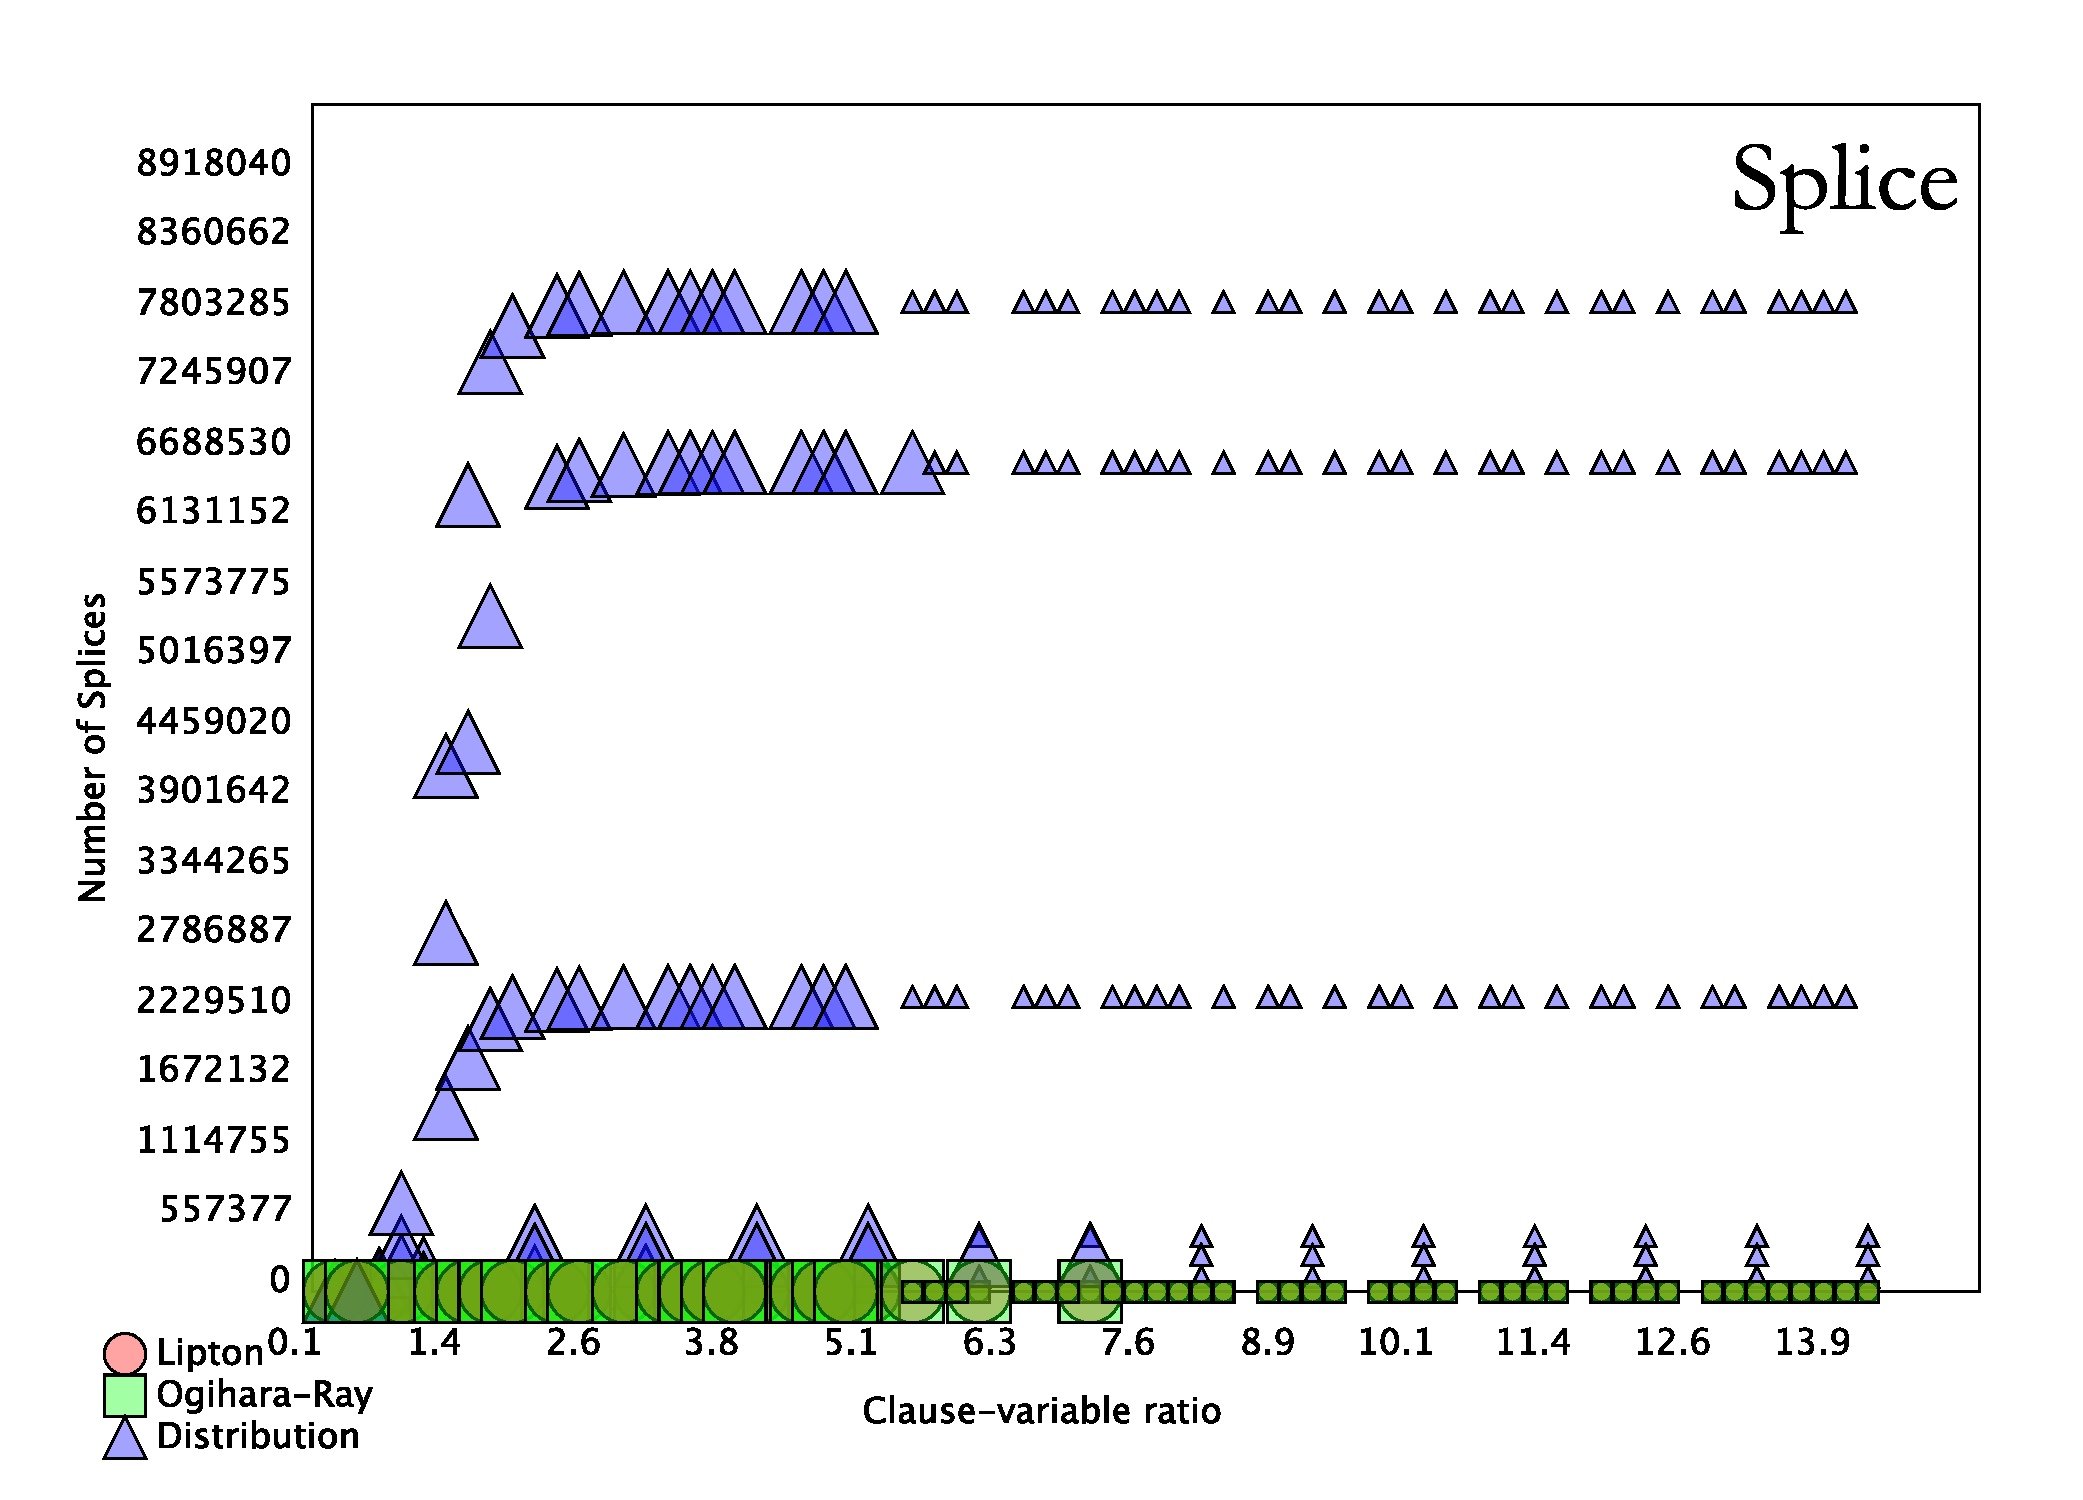
\includegraphics[width=1.1\textwidth]{./figures/metricOutput/Splice.pdf}

\caption{Clause to variable ratio $\alpha$ vs. Number of splices }
\label{spliceFig}
\end{center}
\end{figure}
%%%%%%%%%%%%%%%%%%%%%%%%%%%%%%%%%
\FloatBarrier

%\subsection{Split}
%%%%%%%%%%%%%%%%%%%%%%%%%%%%%%%%%
\begin{figure}[htdp]

\reversemarginpar{

\textbf{Split} portions a tube into two exact tubes.\\

The Distribution algorithm requires a linear number of splits.\\

Lipton's and Ogihara-Ray's algorithms are constant in splits based the number of variables.
 }

\begin{center}

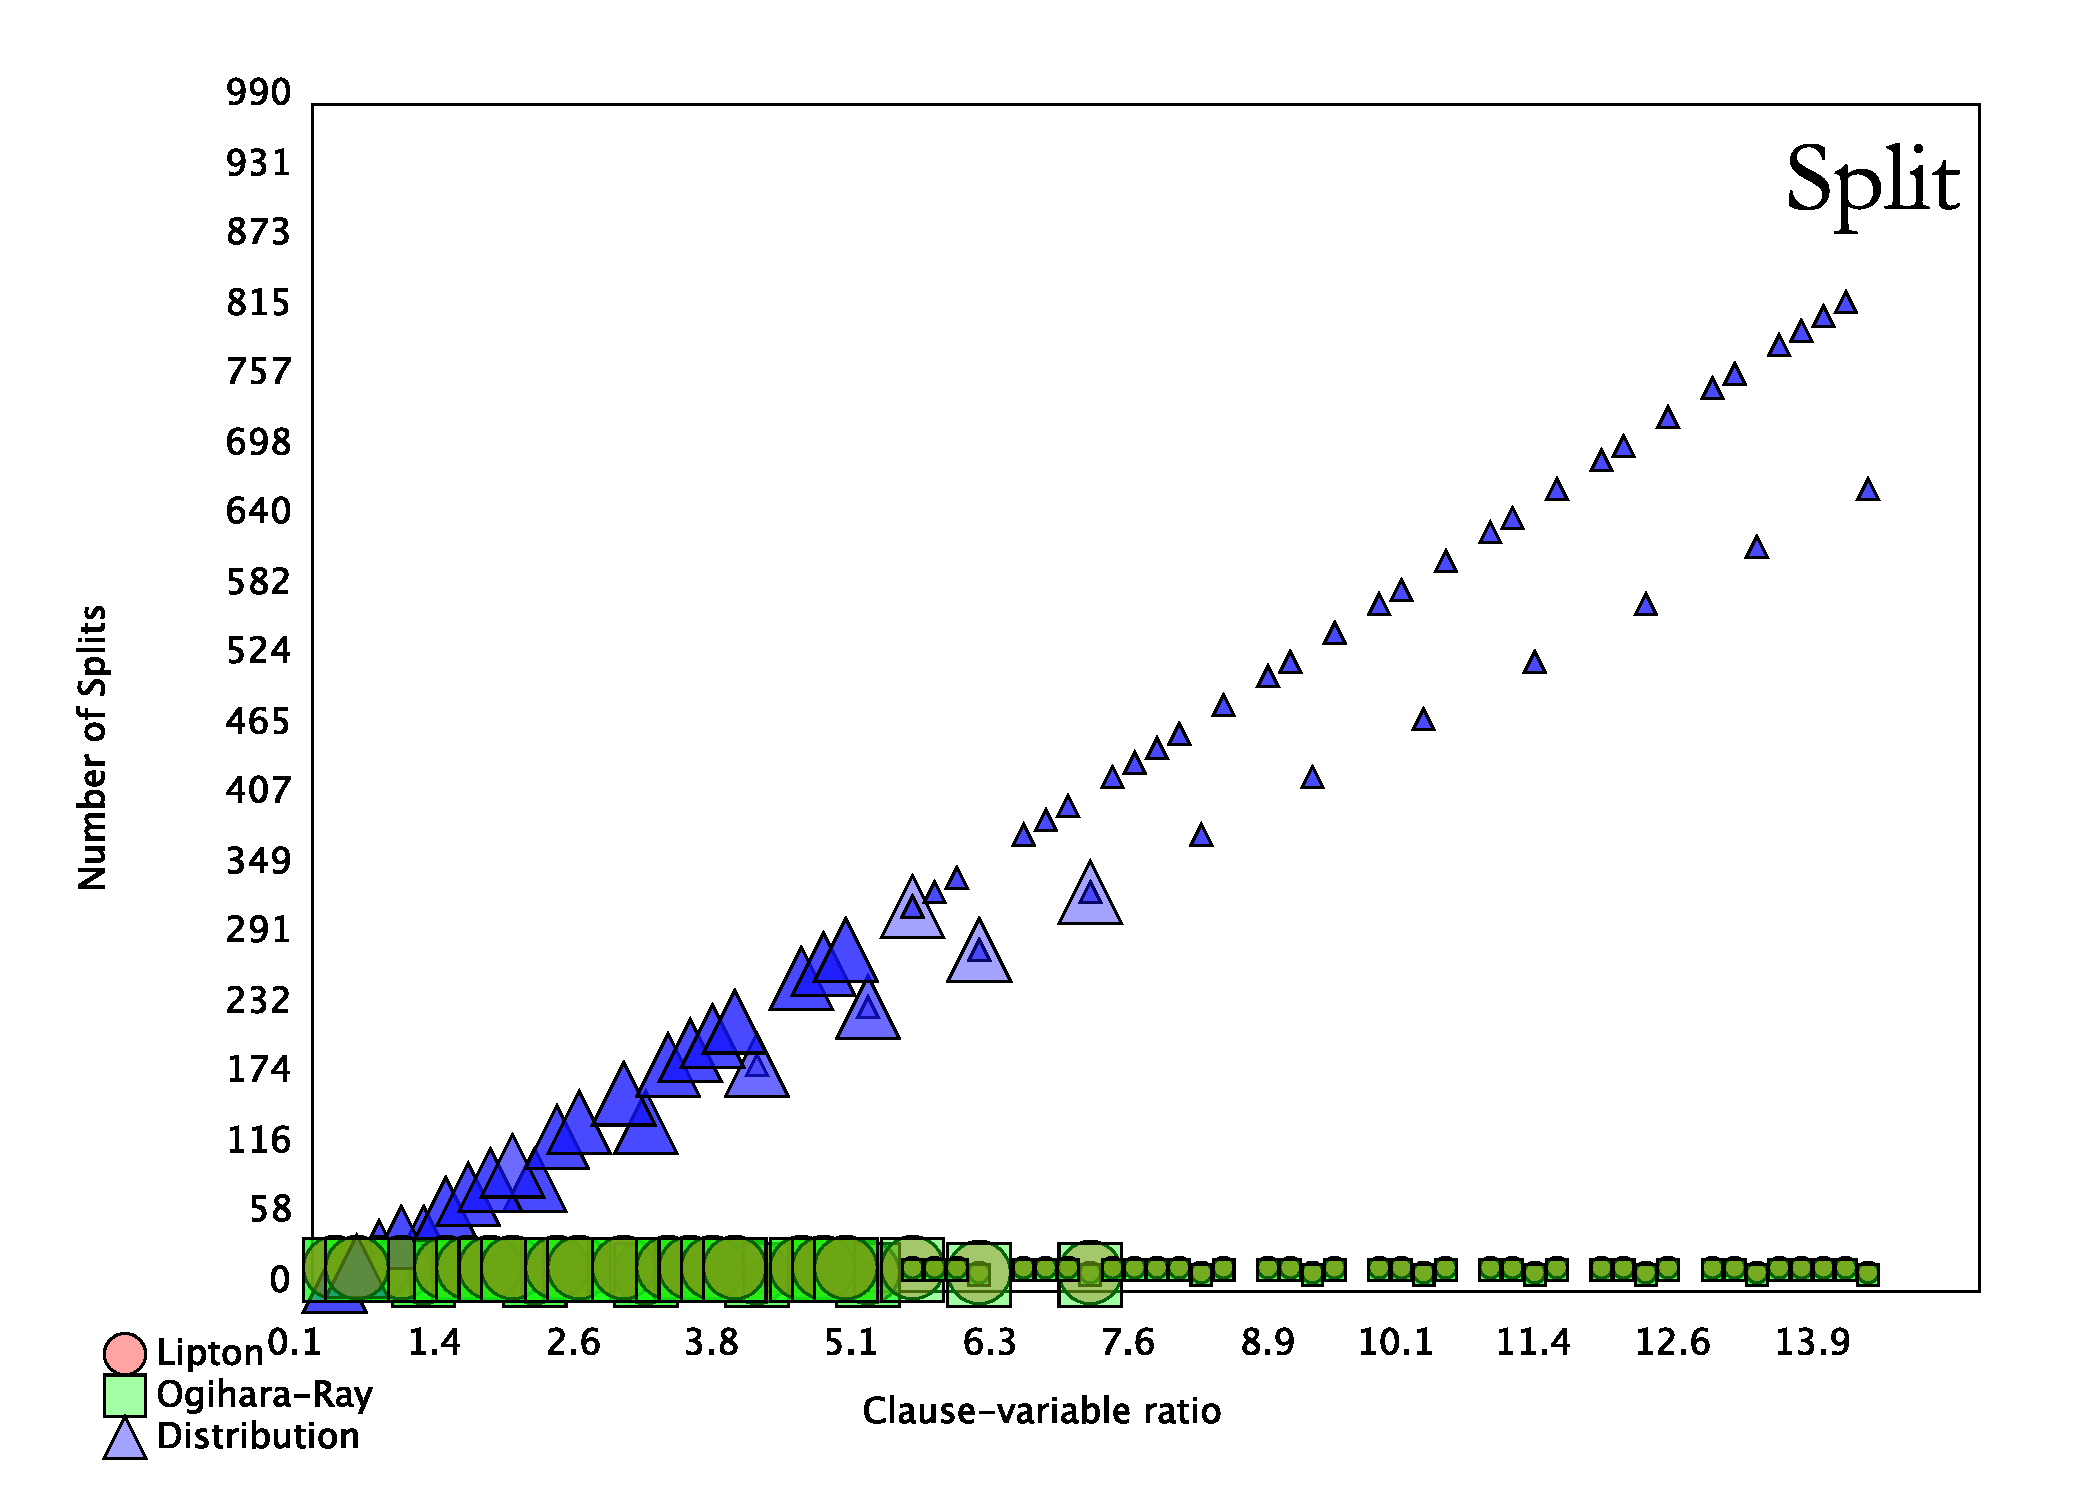
\includegraphics[width=1.1\textwidth]{./figures/metricOutput/Split.pdf}

\caption{Clause to variable ratio $\alpha$ vs. Number of splits }
\label{splitFig}
\end{center}
\end{figure}
%%%%%%%%%%%%%%%%%%%%%%%%%%%%%%%%%
\FloatBarrier

			
%\subsection{Time}
%%%%%%%%%%%%%%%%%%%%%%%%%%%%%%%%%
\begin{figure}[htdp]

\reversemarginpar{
\textbf{Time} measures algorithm execution time in seconds.\\

Ogihara-Ray's algorithm requires the least time.  In cases where the {\sc Satisfiability} instance is under-constrained, where more possible solutions occur, the algorithm takes the greatest time.  Less pruning occurs in over-constrained instances, reducing the execution time of test instances.\\

Lipton's algorithm executes in exponential time $\alpha \approx [4.2, 8.2]$ (the phase transition region for 3-{\sc Sat}) taking the longest.\\

The Distribution algorithm executes in exponential time, and performs better than Lipton's algorithm for low conflict ratios.  However over the entire sweep performs worse than both Lipton's and Ogihara-Ray's algorithms.  It shares the same $\alpha \approx [4.2, 8.2]$ during the $3$-{\sc Sat} phase-transition.
}

\begin{center}

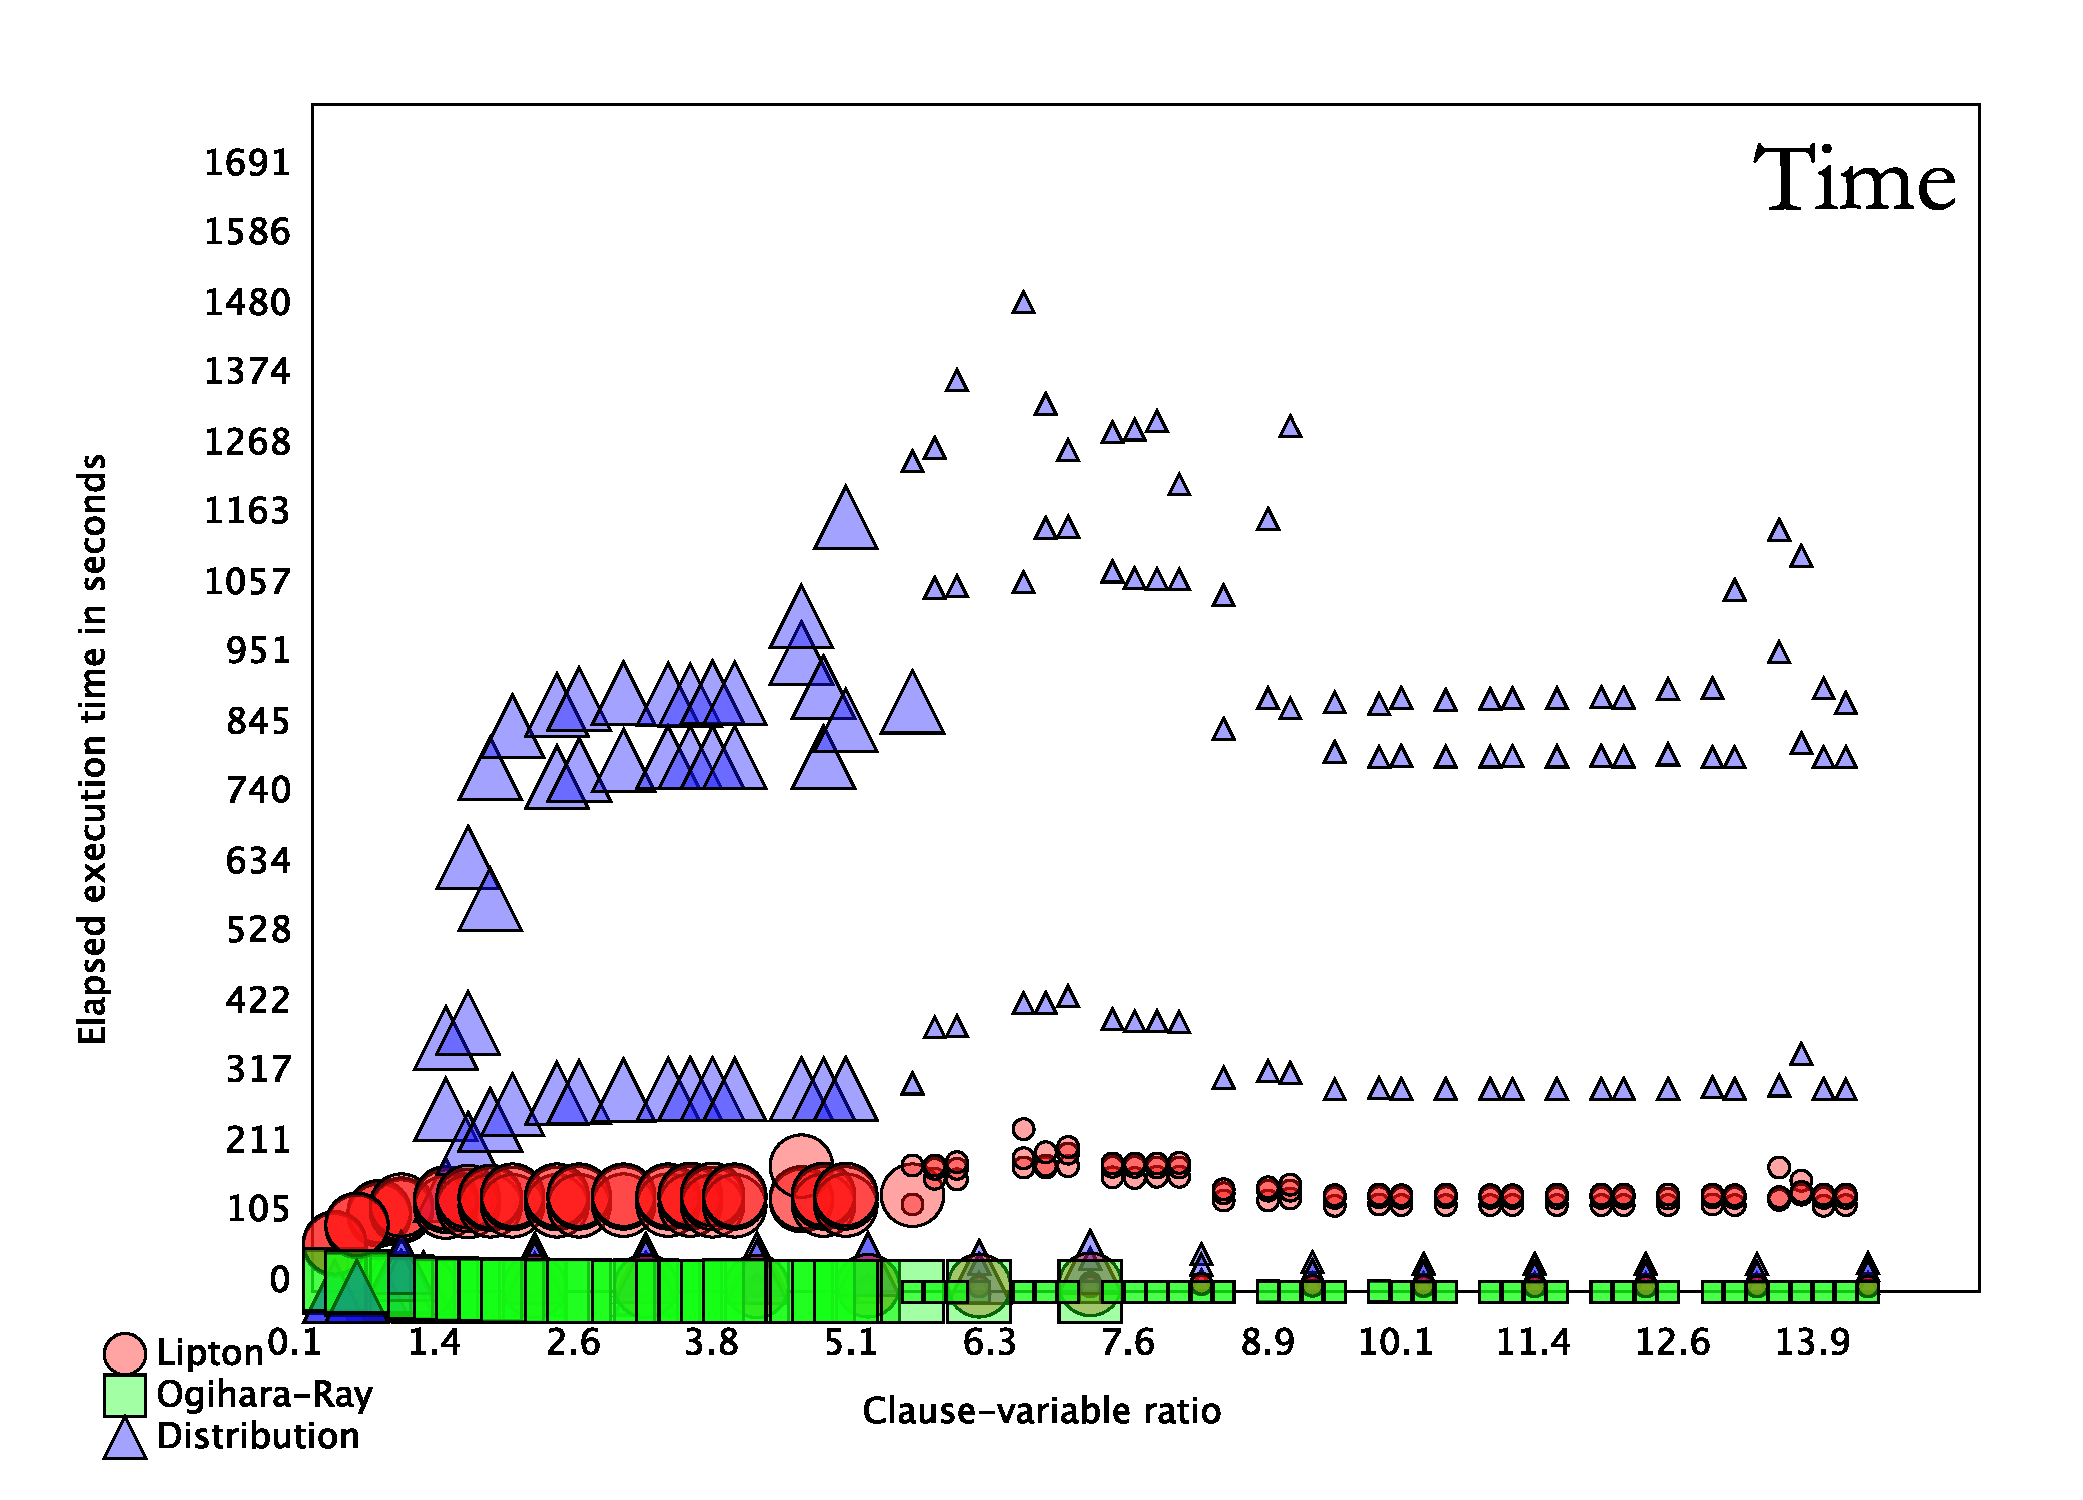
\includegraphics[width=1.1\textwidth]{./figures/metricOutput/Time.pdf}

\caption{Clause to variable ratio $\alpha$ vs. execution time in seconds }
\label{timeFig}
\end{center}
\end{figure}
%%%%%%%%%%%%%%%%%%%%%%%%%%%%%%%%%

\FloatBarrier
			
%\subsection{Solution space}
%%%%%%%%%%%%%%%%%%%%%%%%%%%%%%%%%
\begin{figure}[htdp]

\reversemarginpar{
\textbf{Memory} measures witness footprint in Bytes.\\

Lipton's and Ogihara-Ray's algorithms share the same solution footprint.\\

The Distribution algorithm contains a larger solution footprint after the trivially satisfiable instances with $\alpha \approx [0.2, 0.8]$.  The space contains a set of non-conflicting assignments from $\alpha \approx [0.8, 2.9]$.  Non-conflicting assignments consist of witnesses for only necessary literals. \\

Each {\sc Satisfiability} instance has a constrained solution space during the phase-transition region.  All three algorithms share the same footprint.  There are no satisfiable instances in this test with $\alpha > 7.2$. The axis in Figure \ref{memoryFig} scales accordingly.
}

\begin{center}

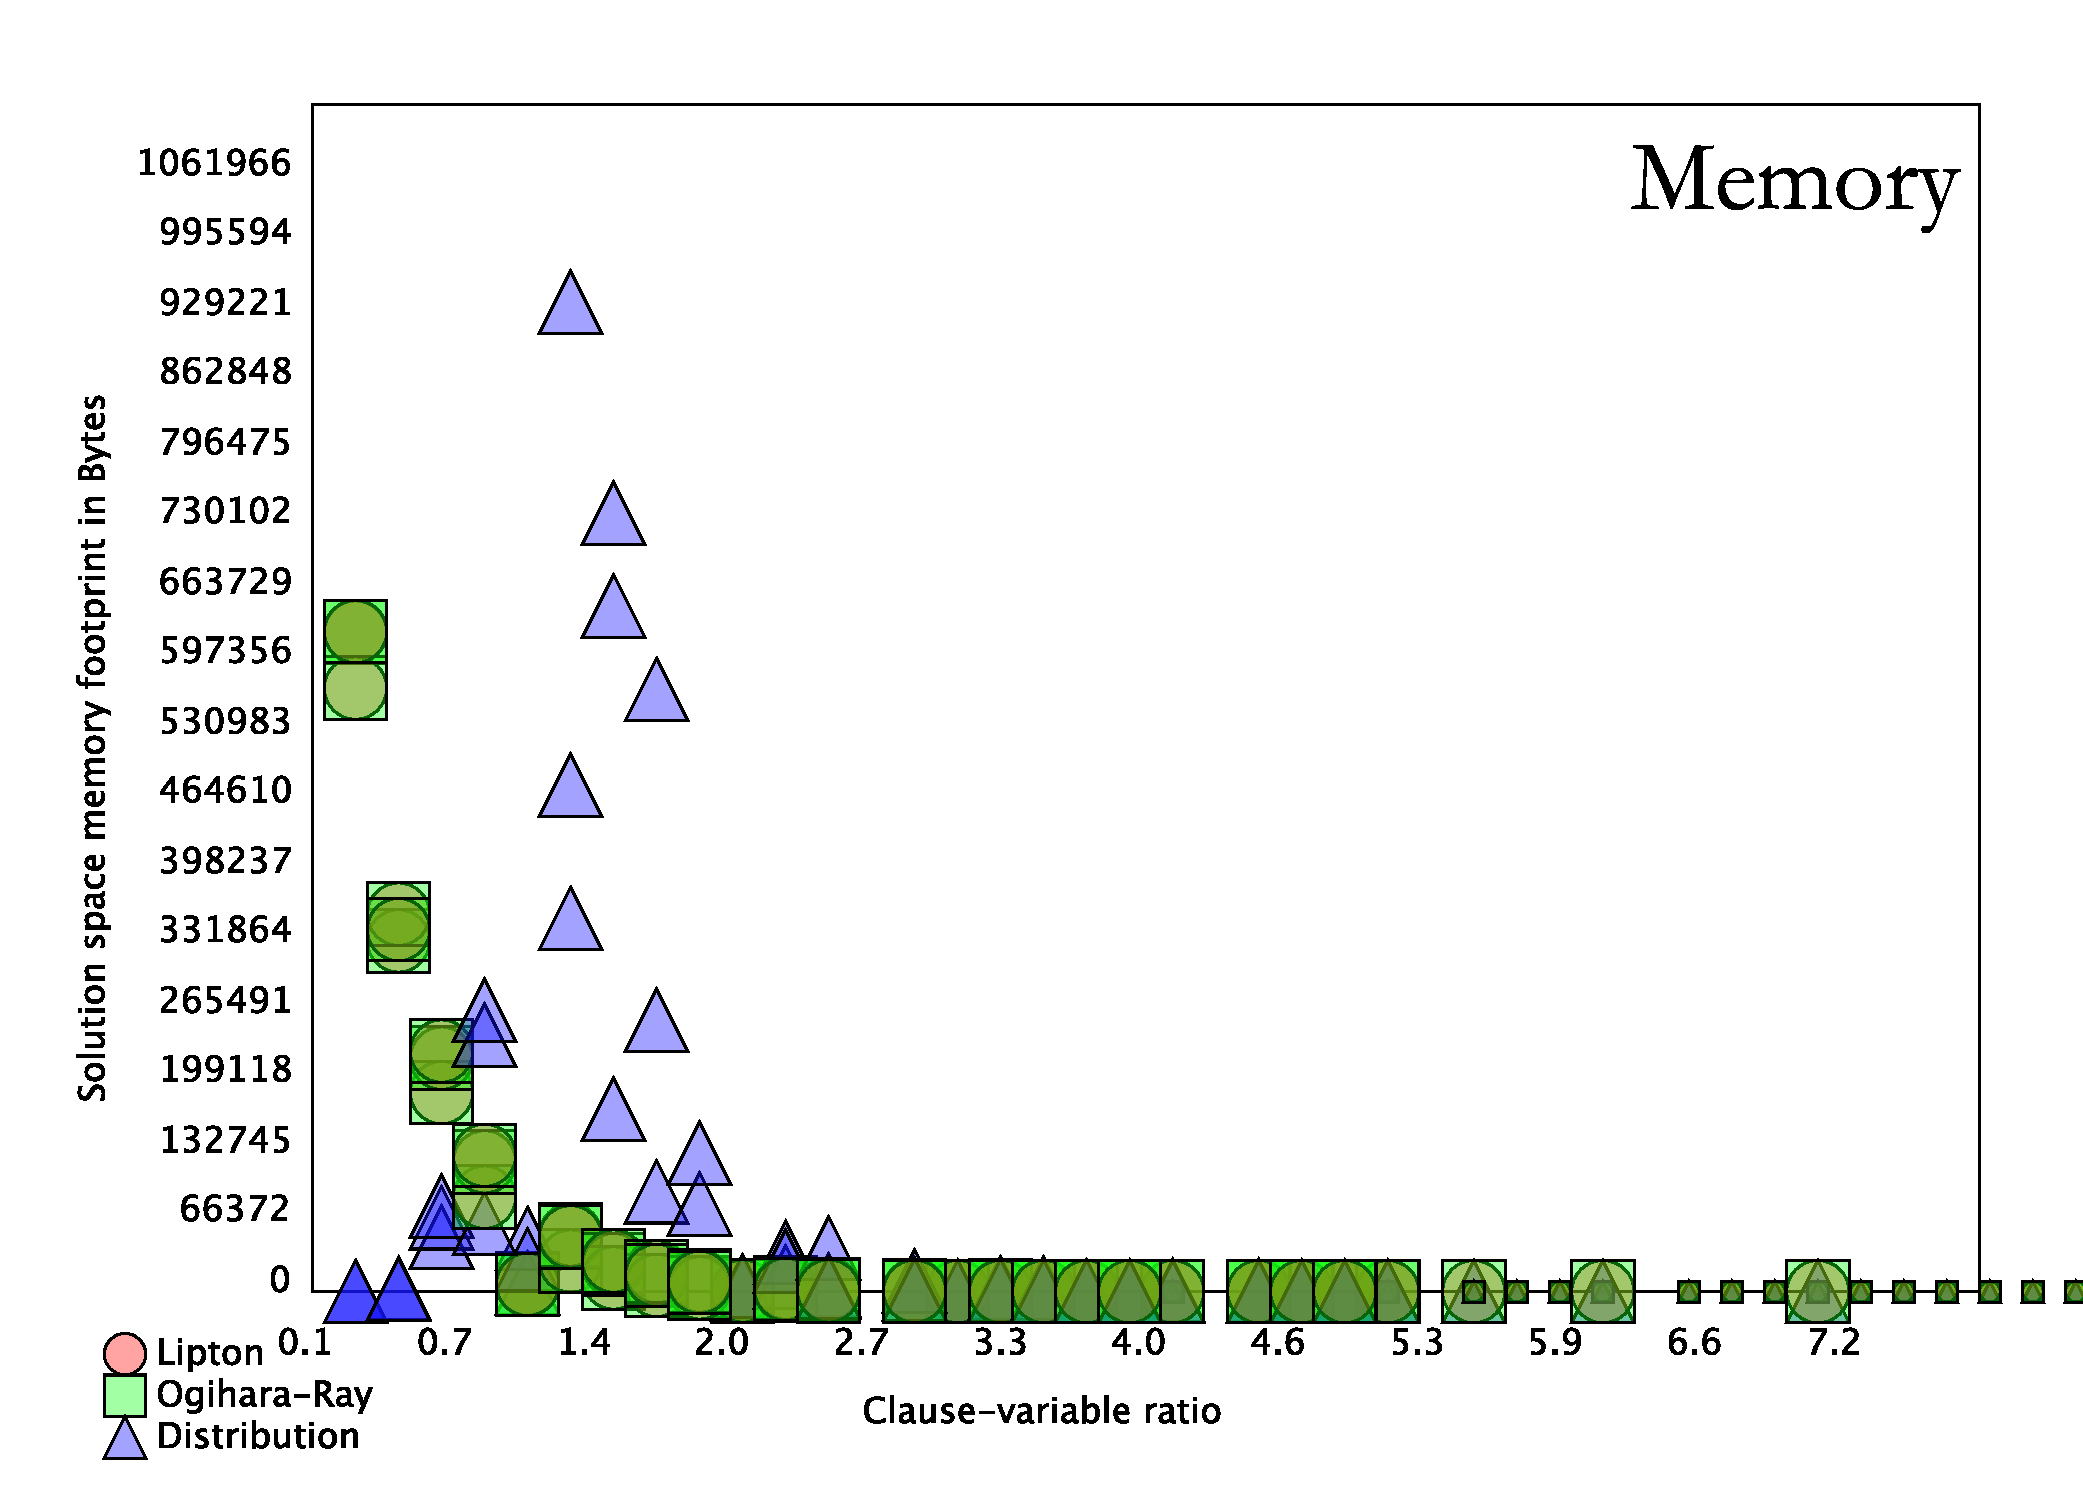
\includegraphics[width=1.1\textwidth]{./figures/metricOutput/Memory.pdf}

\caption{Clause to variable ratio $\alpha$ vs. satisfiable solution footprint in Bytes }
\label{memoryFig}
\end{center}
\end{figure}
%%%%%%%%%%%%%%%%%%%%%%%%%%%%%%%%%

\FloatBarrier
